% !TeX root = ..\discrete_math.tex
\chapter{Теория графов}
\section{Основные определения}
Пусть $M$ и $N$ - два конечных множества. Будем называть пару множеств $\langle M, N \rangle$ \textbf{ориентированным графом}.
При этом элементы множества $M$ называются \textbf{вершинами} графа, элементы множества $N$ - \textbf{дугами} графа. 
Граф, у которого направления соединения не определены, называется \textbf{неориентированным графом}. В них
соединения называются \textbf{ребром}, а вершина - \textbf{узлом}.

\begin{figure*}[!h]
    \centering
    \begin{minipage}[t]{4cm}
        \centering
        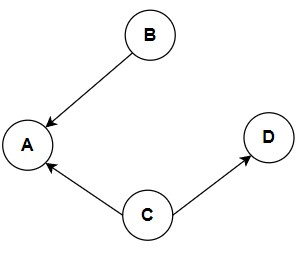
\includegraphics{graph_or.jpg}
        \caption{Ориентированный граф}
    \end{minipage}
    \hspace{3cm}
    \begin{minipage}[t]{4cm}
        \centering
        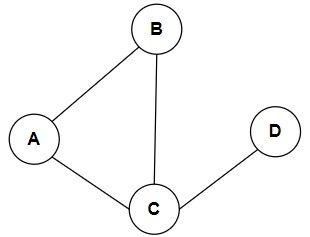
\includegraphics{graph_nor.jpg}
        \caption{Неориентированный граф}
    \end{minipage}
\end{figure*}

\textbf{Степенью} называется количество ребер, соединенных с этой вершиной.
Если степень вершины равна 0, то такая вершина называется \textbf{изолированной}.
Степень вершины может быть \textbf{входящая} и \textbf{исходящая}. Входящая степень вершины $v$
это количество ребер вида $\langle i, v \rangle$, то есть количество ребер которые входят в $v$.
Исходящая степень вершины $v$ это количество ребер вида $\langle v, i \rangle$, то есть количество ребер
которые входят из $v$.

\begin{thm}
    В любом графе всегда найдутся хотя бы две вершины с одинаковой степенью.
\end{thm}

Дуга, у которой начало и конец совпадают, называется \textbf{петлей}.

Граф $\langle M', N'\rangle$ называется \textbf{простым путем}, если
\begin{enumerate}
    \item число его дуг $k$ на единицу меньше числа вершин
    \item можно так пронумеровать $M'$ числами от 0 до $k$ и $N'$ числами от 1 до $k$,
    что для любой дуги $u \in N'$
\end{enumerate}

Пусть $num$ - это получение номера дуги или вершины, а $beg(u)$ и $end(u)$ начало и конец дуги 
$u$ соответственно. Тогда для любой дуги $u$ в графе верно выражение:
\begin{equation}
    \label{simple_path}
    num(u) = num(end(u)) = num(beg(u)) + 1
\end{equation}
Различие между \textbf{путем} и \textbf{простым путем} заключается в том, что во втором случае
недопустимы повторы вершин и дуг в пути.
\begin{figure}[h]
    \centering 
    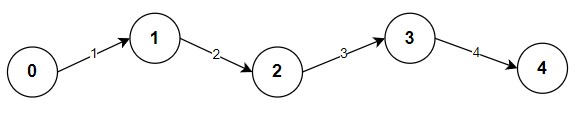
\includegraphics{simple_path.jpg}
    \caption{Простой путь}
\end{figure}

Граф $\langle M', N'\rangle$ называется \textbf{цепью}, если:
\begin{enumerate}
    \item число его дуг $k$ на единицу меньше числа вершин
    \item можно так пронумеровать $M'$ числами от 0 до $k$ и $N'$ числами от 1 до $k$,
    что для любой дуги $u \in N'$
\end{enumerate}
То есть, он включает либо условие простого пути \ref{simple_path}, либо
\begin{equation}
    \label{chain}
    num(u) = num(end(u)) + 1 = num(beg(u))
\end{equation}
Дуги, для которых выполняется \ref{simple_path}, принято называть \textbf{положительно ориентированными},
а те, для которых выполняется \ref{chain} \textbf{отрицательно ориентированными}.

\begin{figure}[h]
    \centering 
    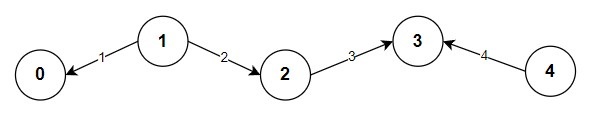
\includegraphics{chain.jpg}
    \caption{Цепь}
\end{figure}

Граф $\langle M', N'\rangle$ называется \textbf{контуром}, если
\begin{enumerate}
    \item число дуг $k$ равно числу вершин
    \item можно так пронумеровать $M'$ и $N'$ числами от 1 до k, что для любой
    дуги $u \in N'$
\end{enumerate}
\begin{equation}
    num(u) \stackrel{\text{mod k}}{=} num(end(u)) \stackrel{\text{mod k}}{=} num(beg(u)) + 1
\end{equation}
Иными словами, контур - это простой путь, где начало и конец совпадают.

\begin{figure}[h]
    \centering 
    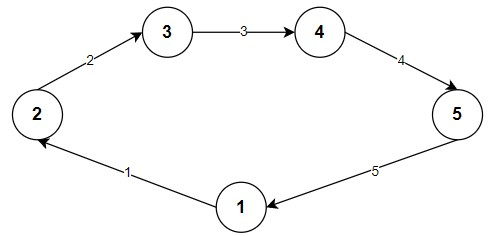
\includegraphics{loop.jpg}
    \caption{Контур}
\end{figure}

\vspace{3mm}

Граф $\langle M', N'\rangle$ называется \textbf{циклом}, если
\begin{enumerate}
    \item число дуг $k$ равно числу вершин
    \item можно так пронумеровать $M'$ и $N'$ числами от 1 до $k$, что для любой дуги $u \in N'$
\end{enumerate}
\begin{equation}
    num(u) \stackrel{\text{mod k}}{=} num(end(u)) \stackrel{\text{mod k}}{=} num(beg(u)) + 1
\end{equation}
либо
\begin{equation}
    num(u) \stackrel{\text{mod k}}{=} num(end(u)) + 1 \stackrel{\text{mod k}}{=} num(beg(u))
\end{equation}
Цикл - это цепь, в которой начало и конец совпадают.
\begin{figure}[h]
    \centering 
    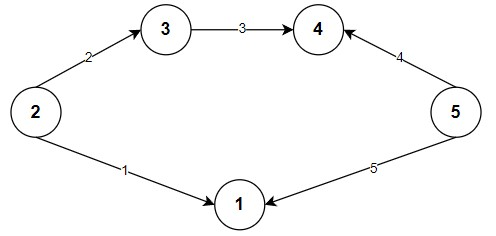
\includegraphics{cycle.jpg}
    \caption{Цикл}
\end{figure}

\section{Связность. Компоненты связности и сильной связности}
Граф $\langle M, N\rangle$ называется \textbf{связным}, если любые две различные его
вершины можно соединить цепью. Любой граф может быть однозначно разделен на максимальные
связные подграфы, которые называют его \textbf{компонентами связаности}.
\begin{figure}[h]
    \centering 
    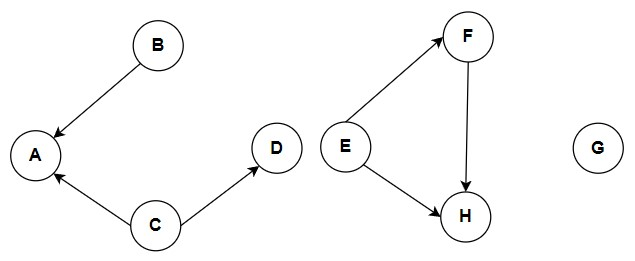
\includegraphics{connectivity.jpg}
    \caption{Пример несвязного графа}
\end{figure}

Граф $\langle M, N\rangle$ называется \textbf{сильно связным}, если любые две различные
вершины A и B можно соединить путем с началом в A и концом в B. В любом графе можно однозначно
выделить максимальные сильно связные подграфы, которые называются его \textbf{компонентами сильной связности}.
\begin{thm}
    Граф компонент сильной связности не имеет контуров.
\end{thm}
